\chapter[Introduction]{Introduction}
\section{Motivation}
Humankind has only a few ways to generate reliable, nonintermittent baseload 
power: fossil fuels, hydro-power, geothermal power, and nuclear energy. 
Because of increasing global climate change concerns, sources with negligible 
CO$_2$ footprints are crucial measures for global temperature control. Thus, 
from an environmental viewpoint, hydro and nuclear power are preferable ways 
to generate reliable power. Nevertheless, the potential for a hydro-power is 
strictly limited by local geographical conditions; hence, the only option left 
is nuclear power. Nuclear power plants provided 10\% of global electricity 
supply in 2018 \cite{iea_nuclear_2019}. Moreover, nuclear share in energy 
generation is projected to stay constant through 2040, while electricity 
demand will increase by 30\% \cite{noauthor_world_2017}. 

The Generation IV International Forum (GIF) chose \glspl{MSR} among the six 
advanced reactor concepts for further research and development. \glspl{MSR} 
offer significant improvements ``in the four broad areas of sustainability, 
economics, safety and reliability, and proliferation resistance and physical 
protection" \cite{doe_technology_2002}. To achieve the goals formulated by the 
GIF, \glspl{MSR} simplify the reactor core and improve inherent safety by 
using liquid coolant which is also a fuel\footnote{Herein \glspl{MSR} are 
assumed to be reactors with liquid fuel which simultaneously serves 
as coolant.}. In a thermal spectrum \gls{MSR}, liquid fuel consists 
of carrier salt (i.e. LiF, LiF-BeF$_2$ or LiF-NaF-KF) and fluorides of fissile 
and/or fertile materials (i.e. UF$_4$, PuF$_3$ and/or ThF$_4$). This fuel  
circulates in a loop-type primary circuit \cite{haubenreich_experience_1970}. 
This innovation leads to immediate advantages over traditional, 
solid-fueled, reactors. These include near-atmospheric pressure 
in the primary loop, relatively high coolant temperature, outstanding 
neutron economy, a high level of inherent safety, reduced fuel 
preprocessing, the ability to continuously remove fission products 
and add fissile and/or fertile elements without shutdown 
\cite{leblanc_molten_2010}. The possibility of continuously removing 
neutron poisons increases the potential fuel burnup and thus 
improves the resource utilization of \glspl{MSR}. Finally, the \gls{MSR} 
also could be employed for transmutation of 
spent fuel from current \glspl{LWR} \cite{fratoni_design_2004}.

Recently, interest in \glspl{MSR} has resurged, with multiple new companies 
pursuing commercialization of \gls{MSR} designs\footnote{Examples 
include liquid-fueled \gls{MSR} designs from Terrapower, Terrestrial, 
ThorCon, Flibe, Copenhagen Atomics, Elysium, etc.}. China's \gls{MSR} program 
was initiated in 2011 and promises to startup a 2MW$_{th}$ 
liquid-fueled test \gls{MSR} in 2020, a 10MW$_{th}$ 
demonstration reactor in 2025, and a gigawatt-level 
commercial reactor in 2050 \cite{zhang_review_2018}. The European 
Union funds the Safety Assessment of the Molten Salt Fast Reactor 
(SAMOFAR) project, in which several European research institutes and 
universities are developing various molten salt reactor prototypes 
such as the \gls{MSFR} \cite{fiorina_molten_2013} and the \gls{MOSART} 
\cite{ignatiev_molten_2014}. To advance these \gls{MSR} concepts, particularly 
concerning their strategies for online reprocessing and refueling, 
we need computational analysis methods capturing their unique reactor physics, 
fuel reprocessing mechanics, and chemistry. 

The main objective of the proposed work is to develop the online 
reprocessing simulation package, SaltProc, which couples with the 
continuous-energy Monte Carlo depletion calculation code, Serpent 2 
\cite{leppanen_serpent_2014}, for liquid-fueled \gls{MSR} depletion 
simulations. Most of existing \gls{MSR} depletion simulators usually assume 100\% 
efficiency of the neutron poison removal process (see Chapter 1). The ultimate 
objective of this effort is to develop a generic open-source tool capable of 
simulating a wide range of liquid-fueled systems --- including two-fluid and
multi-region designs --- and to validate it against existing modeling efforts. 
Moreover, SaltProc enables poison extraction simulation based on a 
realistic physics-based fuel processing model.

This document outlines the motivation, preliminary work, and future work 
proposed towards developing a simulation tool for analyzing fuel depletion in 
a liquid-fueled \glspl{MSR}. Chapter 1 serves as a literature review, 
providing background on fuel burnup, online fuel reprocessing approaches, 
safety parameter evolution during reactor operation, and how these 
concepts have been applied to a wide range of \glspl{MSR} in the literature. 
Chapter 2 covers modeling online reprocessing details and proposed computation 
tool architecture. Chapter 3 explains the \gls{VV} method, demonstration 
cases, and safety parameter evolution. Specifically, these demonstration and 
verification efforts will focus on the \gls{TAP} \gls{MSR} because it is well 
analyzed in the literature. Chapter 4 gives the safety parameter overview and 
outlines the plan for analyzing these parameters' evolution during \gls{TAP} 
reactor lifetime. Finally, remaining future work and expected contributions to 
the nuclear community are summarized in Chapter 5.

\section{Fuel burnup and online reprocessing}
All liquid-fueled \gls{MSR} designs involve varying levels of online fuel 
processing. Minimally, volatile gaseous fission products (e.g., Kr, Xe) 
escape from the fuel salt during routine reactor operation and must be 
captured. Additional systems might be used to enhance the removal of those 
elements. Most designs also call for the removal of rare earth metals from 
the core since these metals act as neutron poisons. Some designs suggest a 
more elaborate list of elements to process (figure~\ref{fig:periodic_tab}), 
including the temporary removal of protactinium from the salt or other 
regulation of the actinide inventory in the fuel salt 
\cite{ahmad_neutronics_2015}. Fresh fuel salt with dissolved fissile and/or 
fertile material (e.g., $^{233}$U, $^{232}$Th, \gls{LEU}, a transuranic 
vector from \gls{LWR} \gls{SNF}) make up the salt mass loss caused by poison 
removal and conserves the total mass in the primary loop.
\begin{figure}[htp!] % replace 't' with 'b' to 
  \centering
  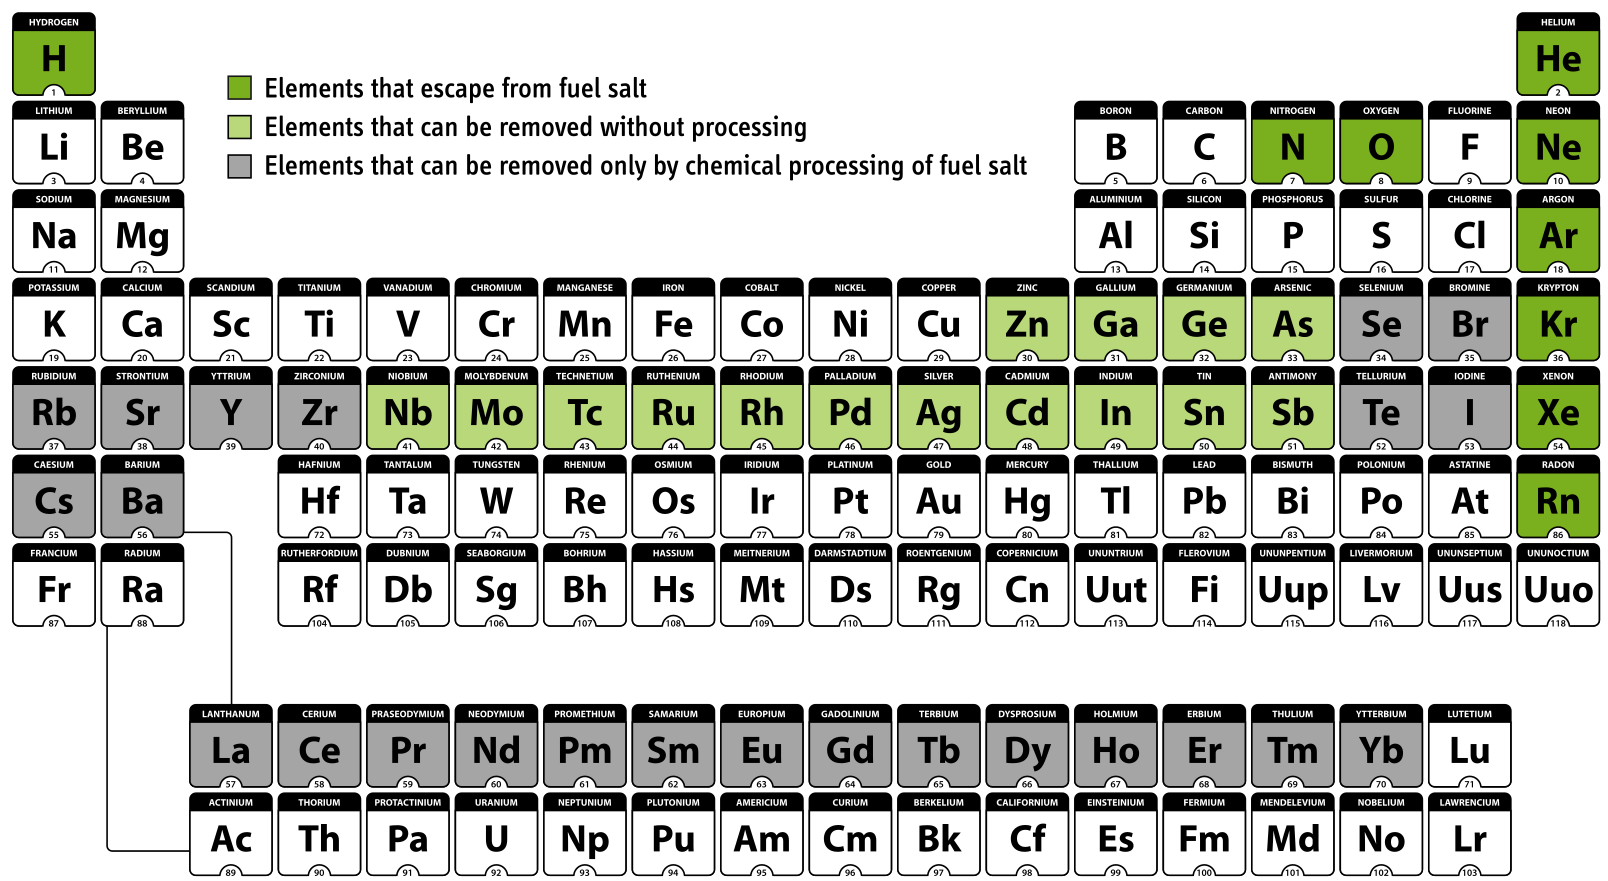
\includegraphics[width=0.9\textwidth]{periodic_map.png}
  \caption{Processing options for \gls{MSR} fuels (figure reproduced from 
  Ahmed \emph{et al.} \cite{ahmad_neutronics_2015}).}
  \label{fig:periodic_tab}
\end{figure}

Most liquid-fueled nuclear reactor concepts adopt nonintermittent separations 
and feeds: the core material is circulated to or from the core at all times 
(continuously) or specific intervals (batch-wise). In contrast, in a 
solid-fueled reactor, fission products and actinides remain within the initial 
fuel material during and after the operation until reprocessing. The ability 
to perform online fuel salt reprocessing improves the potential neutronics 
performance of liquid-fueled reactors. First, liquid-fueled reactors can 
operate with a relatively small excess reactivity because fissile material is 
continuously being added to the core. Second, continuously 
removing fission products, including strong absorbers (poisons) should 
significantly improve fuel utilization and decrease parasitic neutron 
absorption. Finally, for a breeder\footnote{\gls{CR} 
$\equiv$ fissile generated/fissile consumed: if CR $<$ 1, the reactor is a 
``converter''; CR $\equiv$ 1, an ``isobreeder''; CR $>$ 1, a 
``breeder.''} excess of fissile material might be continuously extracted  
from the core and used to start up new reactors. Nevertheless, the removal of 
each element from the liquid fuel salt presents a unique challenge in terms of 
chemical separation, storage, and disposal of the separated materials.

Continuous fuel salt reprocessing prevents the usage of most contemporary 
nuclear reactor fuel burnup software. To handle the material flows and 
potential online removal and feed of liquid-fueled systems, early \gls{MSR} 
simulation methods at \gls{ORNL}, which integrated neutronic and fuel cycle 
codes (i.e., Reactor Optimum Design (ROD) \cite{bauman_rod_1971}) into 
operational plant tools (i.e., Multiregion Processing Plant (MRPP) 
\cite{kee_mrpp_1976}) for \gls{MSR} fuel reprocessing system design. A summary 
of recent efforts is listed in table~\ref{tab:msr_codes}.
\begin{table}[t]
\fontsize{9}{11}\selectfont
\caption{Tools and methods for liquid-fueled \glspl{MSR} fuel salt depletion 
analysis.}
\begin{tabularx}{\textwidth}{X X X X X} 
\hline 
&Nuttin \emph{et al.}, 2005 \cite{nuttin_potential_2005}& Aufiero \emph{et al.}, 
2013 \cite{aufiero_extended_2013} & Betzler \emph{et al.}, 2018 
\cite{betzler_fuel_2018}&Proposed work \\ [12pt]
\hline
Neutron transport software & \gls{MCNP} & Serpent 2 & SCALE6.2 & Serpent 2 \\ 
[12pt]
Neutron transport method & \multicolumn{2}{c}{Monte Carlo continuous energy} & 
Deterministic discrete ordinates & Monte Carlo continuous energy \\ [12pt]
Burnup software & REM & Serpent 2 & ORIGEN-S & Serpent 2 \\ 
[12pt]
Geometry model & unit cell & full-core 3D & unit cell & full-core 3D\\ [12pt]
\gls{FP} removal/feed  & continuous &continuous & batch-wise & batch-wise\\ 
[12pt]
Separation efficiency &\multicolumn{3}{c}{fixed, must be defined by user 
before simulation} & variable of many parameters \\ [12pt]
Fuel reprocessing plant & \multicolumn{3}{c}{single component, ``black'' box 
model} & realistic multi-component model \\ [12pt]
Reactivity control & \multicolumn{2}{c}{continuous adjustment of fissile 
material injection} & batch injection of fissile material & periodical 
adjustment of geometry and fissile material injection\\
\hline
\end{tabularx}
  \label{tab:msr_codes}
\end{table}

Two main online reprocessing simulation approaches are commonly used in the 
literature: continuous and batch-wise. In the batch-wise approach, the burnup 
simulation stops at a given time and restarts with a new liquid fuel 
composition (after removal of discarded materials and addition of 
fissile/fertile materials). 

Accounting for continuous removal or addition of material presents a greater 
challenge since it requires adding a term to the Bateman equations. In 
SCALE/TRITON, ORIGEN \cite{gauld_isotopic_2011} solves a set of the Bateman 
equations using one-group averaged fluxes and cross sections obtained from a 
transport calculation. The Bateman equations describe the rate of change of 
each isotope, $i$, due to neutron induced reactions and decay processes
\cite{tsoulfanidis_nuclear_2013}:
\begin{align} \label{eq:bateman}
\frac{dN_i}{dt} &= \sum_{m=1}^{M}l_{im}\lambda_mN_m + 
\phi\sum_{m=1}^{M}f_{im}\sigma_mN_m - (\lambda_i + \phi\sigma_i + r_i - 
f_i)N_i + F_i\Big|{i\in [1,M]}\\
& \qquad\qquad (1) \qquad\qquad\qquad (2) \qquad\qquad(3) \quad (4)  \quad 
(5) \quad (6)
\nonumber
\intertext{where}
N_i &= \mbox{atom density of nuclide i} \nonumber \\
M &= \mbox{number of nuclides} \nonumber \\
l_{im} &= \mbox{fraction of decays of nuclide m that result in formation of 
nuclide i}\nonumber \\
\lambda_i &= \mbox{radioactive decay constant of nuclide i} \nonumber \\
\phi &= \mbox{neutron flux, averaged over position and energy} \nonumber \\
f_{im} &= \mbox{fraction of neutron absorption by nuclide m leading to the 
formation of nuclide i} \nonumber \\
\sigma_m &= \mbox{average neutron absorption cross section of nuclide m} 
\nonumber \\
r_i &= \mbox{continuous removal rate of nuclide i from the system} \nonumber \\
f_i &= \mbox{continuous feed rate of nuclide i} \nonumber \\
F_i &= \mbox{production rate of nuclide i directly from fission}\nonumber
\end{align}
The four terms on the right-hand side of the equation represent:
\begin{enumerate}[label=(\arabic*)]
	\item production of species $i$ as a result of the decay of all the 
	nuclides present;
	\item production of species $i$ as a result of neutron capture by all 
	nuclides present;
	\item loss of nuclide $i$ through its own decay;
	\item loss of nuclide $i$ as a result of neutron capture;
	\item loss of nuclide $i$ through continuous removal from the system;
	\item gain of nuclide $i$ as a result of continuous feed to the 
	system.
\end{enumerate} 

Recently, Nuttin \emph{et al.} developed in-house depletion code REM which 
directly couples with \gls{MCNP} \cite{noauthor_mcnp_2004} to simulate fuel 
salt material evolution in a simplified \gls{MSBR}-like reactor. That work 
directly integrated the Bateman differential equations using neutron flux from 
the \gls{MCNP}, tracking all the isotopes available in the data library, and 
control reactivity to maintain reactor critical \cite{nuttin_potential_2005}.

In a similar vein, Aufiero \emph{et al.} extended Serpent 2 for continuous 
reprocessing simulations by explicitly introducing ``reprocessing'' time 
constants into the system of Bateman equations and adding effective decay and 
transmutation terms for each nuclide \cite{aufiero_extended_2013}. The 
developed extension directly accounts for the effects of online fuel 
reprocessing on depletion calculations and features a reactivity control 
algorithm. The extended version of Serpent 2 was assessed against a dedicated 
version of the deterministic ERANOS-based EQL3D procedure in 
\cite{fiorina_investigation_2013} and applied to analyze the \gls{MSFR} fuel 
salt isotopic evolution.

\gls{ORNL} researchers have developed ChemTriton, a Python script for
SCALE/TRITON which uses the batch-wise approach to simulate a continuous 
reprocessing and refill for either single or multiple fluid designs. 
ChemTriton models salt treatment, separations, discharge, and refill using a 
unit-cell MSR SCALE/TRITON depletion simulation over small time steps to 
simulate continuous reprocessing and deplete the fuel salt 
\cite{powers_new_2013, betzler_fuel_2018}.

Most of the existing tools represented fuel salt reprocessing plant as an 
invariable ``black box'' model which removes target elements all at once with 
a fixed efficiency, determined by the user before starting the depletion 
simulation. Typically, such a ``black box'' model is characterized by vector of  
removing elements and their extraction efficiencies:
\begin{equation}
\begin{bmatrix}
N^{in}_{0} \\ \vdots \\ N^{in}_{e} \\ \vdots \\ N^{in}_{E} \\
\end{bmatrix} 
\times
\begin{bmatrix}
\epsilon_{0} \\ \vdots \\ \epsilon_{e} \\ \vdots \\ \epsilon_{E} \\
\end{bmatrix} =
\begin{bmatrix}
N^{out}_{0}\\ \vdots \\ N^{out}_{e} \\ \vdots \\N^{out}_{E}  \\
\end{bmatrix}
\end{equation}
where $N^{in/out}$ is the number density of atoms and $\epsilon$ is the 
extraction efficiency for all elements $e$ in $(0, E)$. The main issues 
related with static ``black box'' model assumptions in the literature include: 
\paragraph{Time-independent separation efficiency vector.} Realistically, 
	long-term reactor operation will require a time-dependent extraction 
	efficiency vector.
\paragraph{The separation efficiency is independent of the reactor operational 
	parameters.} In reality the extraction efficiency depends on temperature, 
	power level, current fuel salt isotopic composition, and material mass 
	flow rate.
\paragraph{All reprocessing plant components are treated as a single ``black 
box'' component.} However, the fuel salt in a reprocessing plant undergoes 
many separate components (e.g., helium bubbling, nickel mesh filter, etc.) 
which target specific elements. Some of these components can be connected in 
series, parallel, or series-parallel. The ``black box'' model (only single 
process) requires massive pre-simulation analytic work from the user to 
calculate lumped separation efficiency vector before a simulation is run and 
cannot be adjusted during the simulation. Additionally, treating the 
processing system as a single ``black box'' may lose dynamics. Finally, the 
waste stream from each component cannot be tracked separately, which is 
necessary for fuel reprocessing system optimization.

Some of the tools listed in table~\ref{tab:msr_codes} used major 
approximations that may lead to inaccurate fuel evolution predictions, and 
others are not available for external users. This work proposes an open-source 
simulation package, SaltProc, which expands the capability of the 
continuous-energy Monte Carlo Burnup calculation code, Serpent 2, for 
simulation liquid-fueled \gls{MSR} operation.

\subsection{Operational and safety parameters evolution} 
\label{sec:saf-par-literature}
In contrast with conventional solid-fueled reactors in which in-core fuel 
residence time is 4-5 years\footnote{For the most common 
18-month cycle, during refueling personnel removing 1/3 of the fuel 
assemblies, re-arranging other assemblies, and loading fresh fuel into the 
core. Thus, each fuel assembly is kept in the core at most $3\times 18=54$ 
months.}, the initial fuel salt batch stays in the \gls{MSR} reactor primary 
loop during the whole lifetime. Therefore, the fuel salt accumulates 
\glspl{FP} not captured by fuel reprocessing system as well as transuranic 
elements\footnote{The chemical elements with atomic numbers greater than 
uranium (92).}. Continuous fuel salt composition evolution has a 
significant influence on the neutron energy spectrum and, consequently, 
affects the reactor behavior, necessitating additional safety analysis.

Nuttin \emph{et al.} studied evolution of a key safety parameter, the 
temperature 
reactivity feedback coefficient, estimating it for the \gls{MSBR} at start-up 
and at equilibrium. The temperature coefficient of reactivity quantifies 
reactivity changes due to temperature increase in the core and was calculated 
in that 
work as:
\begin{align}\label{eq:feedback}
& \qquad\qquad\qquad \alpha = \frac{k_{1200} - k_{900}}{\delta T} 
\intertext{where}
k_{900}, k_{1200}  &= \mbox{the multiplication coefficients at 900K and 
1200K, respectively} 
\nonumber \\
\delta T &= 1200K-900K.\nonumber
\end{align}
That work showed that the \gls{FTC} at start-up and at equilibrium is $-1.5$ 
and $-1.0pcm/K$, respectively. Percent mille ($pcm$) is the unit of reactivity 
equal to $10^{-5}$ of $k_{eff}$.
Nuttin \emph{et al.} also reported a positive and time-invariant 
total temperature coefficient ($+0.8pcm/K$) \cite{nuttin_potential_2005}. 
Recently, Park and colleagues expanded that approach to a full-core 
high-fidelity \gls{MSBR} model and estimated safety parameters evolution over 
20 years of operation \cite{park_whole_2015}. These calculations showed 
relatively large negative total temperature coefficient during 20 years of the 
reactor operation; the coefficient magnitude weakens from $-3.21$ to 
$-1.41pcm/K$ at start-up and at equilibrium composition, respectively. 
Additionally, that work reported control rod worth deterioration from 
$2099pcm$ to $1970pcm$ due to neutron spectrum hardening during reactor 
operation. 

More recently, Betzler \emph{et al.} \cite{betzler_assessment_2017} reported 
key safety parameters evolution for the \gls{TAP} \gls{MSR}: the fuel 
reactivity coefficient at \gls{BOL} and 15 years from \gls{BOL} is negative 
and decreasing slowly over the reactor lifetime; the moderator reactivity 
coefficient is small and positive at \gls{BOL} and became negative after 15 
years of operation. Overall, thermal feedback seems to be stronger in the 
\gls{TAP} reactor and deteriorates insignificantly during the reactor 
operation. Notably, the authors ignored material density change with 
temperature to simplify temperature coefficients calculation; thus, only  
Doppler broadening was taken into account. Finally, the researchers reported 
the total worth of all control rods in the \gls{TAP} core at start-up only. 

The evolution of control rod worth in the \gls{TAP} has not been reported in 
the literature before. The proposed work will illuminate the evolution of majo 
safety parameters (fuel, moderator and total temperature coefficient, void 
reactivity coefficient, control rod worth) for the \gls{TAP} \gls{MSR} at 
various moments during the reactor operation. Additionally, the impact of 
neutron poison accumulation (e.g., $^{135}$Xe) in the fuel salt during 
short-term transients (i.e., load following) on safety characteristics will be 
investigated.

\section{Background Summary}
State-of-the-Art software packages for depletion analysis and evolution of 
safety parameters in liquid-fueled \gls{MSR} are reviewed in this Chapter. 
Based on this summary, I have identified a few possible directions for 
the improvement of \gls{MSR} tools:
\paragraph{Reproducibility/Availability.}
Serpent is the only contemporary nuclear 
contemporary nuclear 
reactor physics software which can perform depletion calculations with taking 
into account online fuel salt reprocessing regimes. However, this built-in 
online reprocessing routine is undocumented  and the discussion forum for 
Serpent users is the only useful source of information at the moment. 
Other mentioned tools are under the closed-source license or available for 
internal users only. These issues can be a barrier to reuse of research 
software and to reproduce scientific results. Thus, a new, open-source, 
reproducible tool for fuel processing simulation would assist in the 
production of reproducible research in the area of liquid-fueled reactor 
modeling.
\paragraph{Realistic fuel reprocessing system model.} 
Major approximations in fuel reprocessing parameters deteriorate fuel salt 
composition predictions since the evolution of safety parameter accuracy is 
strongly dependent on fuel salt composition. A realistic fuel reprocessing 
system model will allow reprocessing component parameter optimization,  
increase fidelity of fuel and waste stream composition calculations, and 
advance reprocessing system design.
\paragraph{Variable extraction efficiency.} Most of the research efforts in 
the literature assumed ideal 100\% extraction efficiency of all removed 
elements, which stayed 
constant during the whole reactor lifetime. But realistically the efficiency 
is time-dependent and changes with respect to operational parameters: 
temperature, power level, salt composition, etc. Thus, the ability to set up 
dynamic separation efficiency must be added in \gls{MSR} simulation tools to 
advance depletion calculations.
\paragraph{Reactivity control.} Reconfigurable moderator configuration in the 
\gls{TAP} core presents a challenge because of the core geometry changes with 
respect to time. The reactivity control module which adjusts the core geometry 
to maintain criticality would be a great capability for simulating a new, more 
advanced \gls{MSR} concepts and short-term transients.
\paragraph{Safety characteristics evolution during reactor operation.} The 
\gls{MSR} fuel salt  accumulates \gls{FP} and transuranic elements which 
significantly shift neutron energy spectrum. Neutron energy hardening might 
worsen the core safety during operation. The impact of the fuel salt evolution 
on the \gls{MSR} safety parameters must be carefully investigated and reported.

The proposed work will hopefully overcome these issues and demonstrate the 
tool capabilities for promising \gls{TAP} \gls{MSR} concept.
